
\chapter{Event Simulation and Reconstruction}\label{sec:simulation}

%%%%%%%%%%%%%
\section{Simulation of Events}
 Vital to the analysis of the data
  gathered using the CMS detector
  are accompanying predictions to be compared against.
 Good predictions can be used not only 
  for direct comparison against data
  as in the case of a cross section measurement,
  but can also be used in the design of 
  future detectors and experiments,
  or for optimizations of parameters in blinded analyses.
 Predictions are made by 
  simulating $pp$ collisions and the subsequent
  decays and interactions that take place
  inside the CMS detector volume
  using Monte Carlo (MC) techniques.
 The first step in producing these simulations
  is the generation of the collision event
  itself, and the second
  is in simulating the interaction of the
  collision products with the detector.

\subsection{Monte Carlo Event Generation}
 There are two complimentary methods used
  in producing a simulation of the 
  collision event, the direct calculation 
  of the scattering amplitude
  (also known as the matrix element, ME),
  and the showering of particles as they
  decay, hadronize and radiate.
 Particles produced in the in the 
  collision before showering
  and hadronization are referred to as prompt.

 As discussed in Section~\ref{sec:protonstructure},
  protons are composite objects which form
  as the result of strong 
  interactions between bound quarks.
 Protons are therefore modeled using 
  parton distribution functions (PDFs)
  which describe the probability of
  finding a given constituent particle,
  or parton, to have a given fraction
  of the momentum of the proton.
 Parton densities vary as a function of the
  energy used to probe the proton and the
  quantity of energy absorbed by the 
  proton is known as the momentum transfer, $Q$.
 The PDF is thus actually a set of density functions,
  one for each parton taken into account
  and for each momentum transfer, 
  and examples of the CTEQ6M parton distribution
  are shown in Figure~\ref{fig:cteqpdfs}.
 Weighted with probabilities from the PDF set
  and summed over,
 MEs are calculated explicitly from Feynman
  diagrams which have initial state particles
  found in the PDF and the desired
  final state. 
 

%%%%%%%%%%%%%
\begin{figure}[htb]
 \center
 \caption[Example Parton Distribution Function from CTEQ6M]{
  Below are proton PDFs shown at two different values of
   momentum transfer, $Q$. 
  The horizontal axis shows the
   momentum fraction carried by the parton
   and the vertical axis shows the parton density.
 } 
 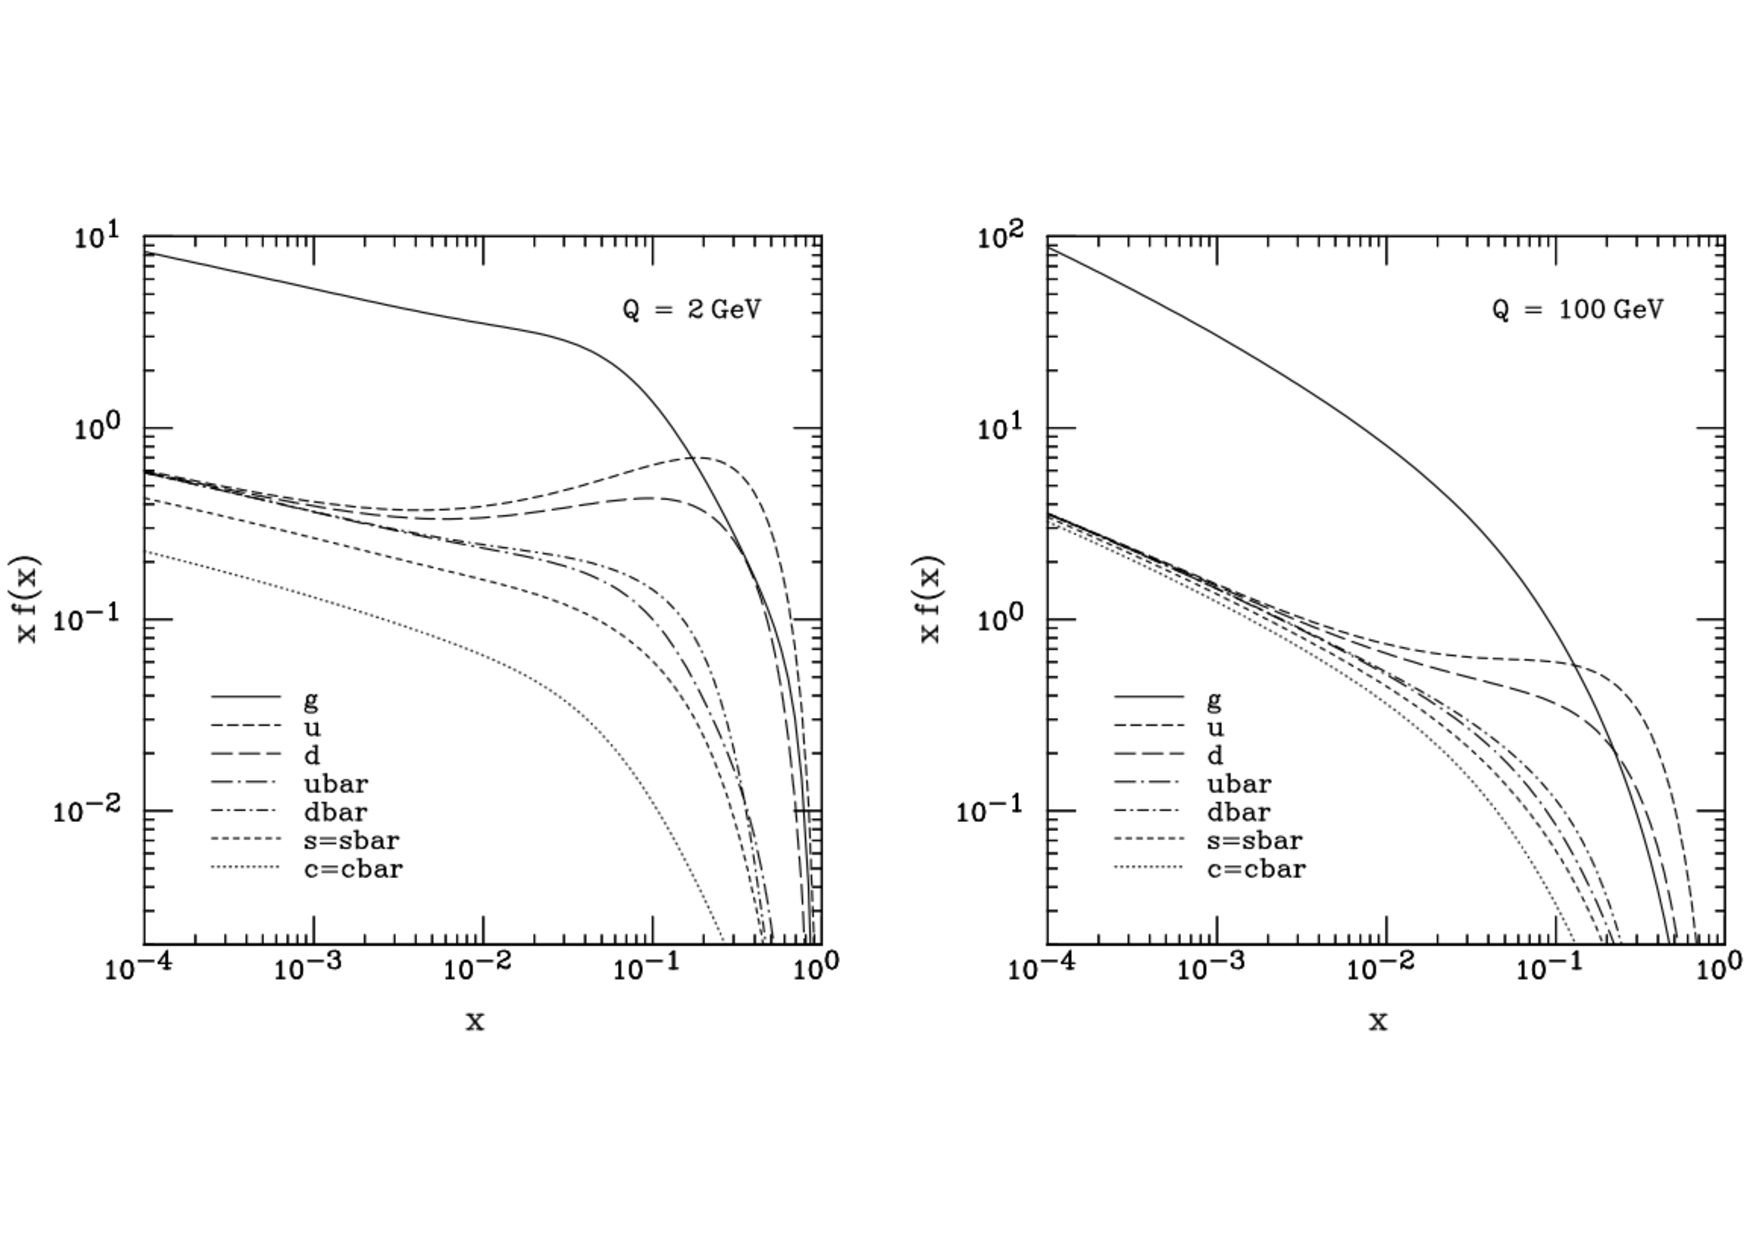
\includegraphics[width=0.9\textwidth]{/Users/rhombus/CMS/Thesis/thesis/pdfs/experiment/cteq_pdf.pdf}
    \label{fig:cteqpdfs}
\end{figure}
%%%%%%%%%%%%%

 Radiation is also important to correctly model.
 At any point in the collision
  any colored particle can radiate a gluon,
  and any charged particle can radiate a photon.
 Gluon radiation from initial state partons is always present
  in $pp$ collisions at the LHC
  and results in jets, columnated showers
  of particles which are the products of quark hadronization
  and gluon splitting.
 The effects of radiation and parton showering are simulated
  using a Markov process in which 
  vertices iteritively are added to partons
  with probabilities based on the
  coupling strengths, energies of the participants
  and the generation of random numbers.
 For the constituents of the proton which
  did not participate in the hard interaction,
  quarks must be created from the vacuum
  to enforce confinement.
 This produces low energy, soft, radiation
  and is known as the underlying event.
 The underlying event must be simulated
  along with the hadronization effects for
  all colored particles.

\subsection{Monte Carlo Generators}

Each of the MC generators used in this
 thesis are designed to serve one of two
 purposes. 
They either calculate MEs for hard
 scattering processes or they compute
 corrections such as hadronization
 or NLO effects.

% The two primary generators used in this
%  thesis are \MADGRAPH/\MADEVENT and \PYTHIA.
% \MADGRAPH is strictly a ME generator
%  which interfaces with \MADEVENT for
%  event generation
%  and \PYTHIA is used for hadronization 
%  and showering.
  
\subsubsection{Matrix Element Calculators}
 For a given $2\rightarrow n'$
  scattering process, the differential cross section is
  a function of the Lorentz-invariant phase space
  as in Equation~\ref{eq:dsigma}.
 To calculate the cross section within 
  a finite phase space, $d\sigma$
  is integrated and 
  \MADGRAPH numerically does this at LO
  through the sampling of random numbers.
 The phase space can be interpreted as a multidimensional 
  hypercube spanning all degrees of freedom
  for all final state particles
  and Equation~\ref{eq:dsigma} is 
  integrated over using the \VEGAS package
  to calculate a weight, $dw$, for each point
  sampled in the phase space.
 The average
  of the weights converges towards $\int dw$.

 To produce events with the frequency
  predicted by the theory being modeled,
  \MADEVENT uses the Von Neumann method to unweight events.
 For each event, a random number, $g$, is generated 
  between 0 and 1 and compared to the ratio
  $dw/dw_{\mathrm{max}}$ where $dw_{\mathrm{max}}$
  is the largest event weight sampled.
 If $dw/dw_{\mathrm{max}}>g$ then the event is kept
  and is otherwise rejected.
 Accepted events generated with \MADGRAPH/\MADEVENT in this 
  way have the same frequency and follow the same
  kinematic distributions as predicted
  from the input Equation~\ref{eq:dsigma}.
   
 A Monte Carlo for FeMtobarn (\MCFM)
  also uses \VEGAS to perform phase space
  integragions, but does so at NLO 
  instead of LO.
 With a much larger phase space to 
  integrate over, \MCFM performs optimizations
  on the integration and produces weighted events.
 With weighted events, an estimation of
  a cross section to NLO accuracy can be made,
  but is made only at the level of partons interacting,
  and in particular does not include corrections
  due to hadronization effects.
 Estimations made by \MCFM thus need to 
  be corrected for hadronization effects
  before being compared with observed cross sections.

\subsubsection{Showering and NLO Corrections}
 Pythia performs hadronization using the
  Lund string model in which quarks are
  confined to the ends of strings and
  gluons are represented as kinks on that string.
 As quarks separate, the string breaks and
  creates a $q\overline{q}$ pair, 
  thus building confinement directly into the model.
 The underlying event is modeled in Pythia
  as a set of $2\rightarrow 2$ processes
  which are correlated with each other via the
  color connections present in the proton.


  and the set of parameters used by Pythia
  to perform calculations is referred to as 
  the tune.
 
 % \subsection{\MADGRAPH}
 % \subsection{Pythia}
 % \subsection{MCFM}
 % \subsection{Powheg}
 % \subsection{FEWZ}
 % \subsection{aMC@NLO}

\subsection{Detector Simulation}

 After events have been produced,
  they are passed to Geant4 
  for simulation of the passage of particles
  through the physical mass of CMS.
 The Geant4 toolkit includes a full
  model of CMS, including 
  all of the subdetectors as well as the
  inert material from the support structure
  and readout electronics.
 The magnetic field is emulated using
  data from measurements on the real field
  and Geant4 uses all of this information
  to register hits in the simulated
  detector as a consequence of the interaction
  between particles produced in the simulated
  event and the simulated material of CMS.
 Additionally, hits are added to the
  simulated detector taking into account
  the rates of background noise, and the
  final output is emulated data
  which is stored in the same way
  as would be data as taken from the real detector.



\section{Reconstruction of Events}\label{sec:reconstruction}

 Real data collected from the detector
  and simulated data output from Geant4
  consist of time-correlated energy deposits
  in the various subdetectors of CMS.
 As a result of the coordinated designs 
  of the subdetectors, the final-state 
  particles which arise from $pp$ collisions 
  at the LHC can be individually identified
  and reconstructed using the combined
  information from the entirity of CMS.
 The associated global event description
  from this particle-flow (PF) reconstruction
  provides excellent performance for
  the identification of electrons and muons,
  as well as for vertex identification
  and the evaluation of \met.
 As a result of the PF reconstruction
  of an event, particles are identified
  and placed into the mutually exclusive
  categories:
  charged and neutral hadrons, photons, 
  electrons and muons.
 
\subsection{Track and Primary Vertex Reconstruction}\label{sec:vertexreco}
 The subdetector closest to the interaction vertex
  is the tracker, which records precise
  information about the trajectories of 
  charged particles as they pass through it.
 Combined with the magnetic field, 
  this allows for the measurement of the
  momenta of these particles as well as a
  means of identifying the the location of
  the primary interaction.

 Tracks are identified via an iteritive process. 
 The first tracks to be reconstructed
  are those which pass strict seeding
  criteria, designed to have a moderate
  efficiency, but negligibly small
  fake rate.
 Then the detector hits associated
  with these tracks are masked
  and the remaining hits are used to
  form track seeds with slightly relaxed
  criteria.
 This operation is repeated, with every
  iteration imposing more complex and time-consuming
  seeding, filtering and track fitting algorithms.
 
% In 2012, the average number of interactions
%  happening at every bunch crossing was 21,
%  and in 2015 it was 
 Because bunches of protons instead of single protons
  are made to cross in the LHC, 
  multiple collisions can take place during the same
  bunch crossing.
 The vertex with the highest scalar sum
  transverse momentum, \pt,
  of tracks and passing further quality selections
  based on the goodness of fit for the tracks
  and the number of tracks associated with a given vertex
  is chosen as the primary vertex (PV).
 The other vertices are referred to as
  pileup vertices and the associated collision
  products as pileup.

 In \ppwbblnbb events, the two $b$ quarks and
  the lepton from the $W$ decay all leave energy
  deposits in the tracker, thus making the choice
  of PV unambiguous.
 However, in the \pploneg events,
  the only visible final state object is a photon,
  and photons do not leave hits in the tracker.
 This makes the identification of the PV
  in the monophoton analysis difficult
  and motivates the using of variables that
  are less sensitive to correct PV identification.
  
\subsection{Electron ID and Reconstruction}

 Electrons are reconstructed using tracker
  hits and ECAL deposits.
 The seed of an electron candidate is selected as 
  an energy deposit in the ECAL with $E_T > 4$ \GeV
  having nearby deposits in the tracker.
 As electrons move in magnetic fields,
  they emit bremsstrahlung radiation
  tangental to their flight path
  and this radiation both appears in the detector, 
  and alters the course of the electron.

 The effects of this radiation are taken
  into account via the Gaussian Sum Filter (GSF)
  track fitting algorithm.
 This algorithm uses weighted sums of Gaussian
  functions to describe electron energy loss
  and thus allows for non-Gaussian corrections
  to the fitting of tracks.
 In the CMS detector, 
  bremsstrahlung from electrons results in the
  emmision of photons in an extended strip
  in the $\phi$ direction and electron
  superclusters (SCs) are made by 
  including the energy deposits from 
  these photons in the ECAL as part of the
  candidate electron object.

 Further requirements during the reconstruction of
  the electron improve the purity of selection.
 The SC and the GSF track are required to 
  be separated by no more than $\abs{\eta}<0.02$
  and $\abs{\phi}<0.15$ and the fraction of
  energy deposited in the HCAL directly behind
  the SC, and the SC is required to be no more
  than 15\%.
 
\subsection{Muon ID and Reconstruction}

 Muon identification is performed using
  two reconstruction and filtering methods to produce 
  `tracker muons' and `standalone muons' which are 
  combined to form  `global muons.'
 Tracker muons are identified starting with
  a track, $\pt>0.5$ \GeV and $p>2.5$ \GeV,
  which is then extrapolated to the muon system.
 If the distance between the the extrapolated
  track and the nearest hit in one of the muon 
  chambers is less than 3 cm, a tracker muon
  is identified.
 Tracker muons are also identified if the 
  pull between the extrapolated track and the
  matched station hit is less than four, where
  pull is defined as the distance between
  the track and the station hit divided by 
  the uncertainties on both measured quanties.
 Tracker muons are built from the inside of the
  detector towards the outside, and 
  standalone muons are built in the other direction.
 Only hits in the muon stations are used to 
  reconstruct standalone muons, with the 
  additional constraint that the path reconstructed
  from the hits points back toward the 
  interaction region.
 Thus, the tracker muon algorithm is well-suited
  for the identification of low-\pt muons by having
  low thresholds and requiring only one track
  and one station hit, while the standalone
  muon algorithm is aimed at high-\pt muons
  which have the energy to penetrate multiple layers
  of muon stations to form tracks which can be
  traced back to the interaction.
 Global muons are required to pass the criteria for both 
  standalone muons and tracker muons, and,
  starting with the standalone muons, 
  the global muon trajectory is refit using information from both 
  the muon stations and the tracker,
  yielding an improved energy resolution than either one.
 %For muons with $\pt<200$ \GeV, the resolution of the tracker

\subsection{Lepton Isolation}

After having been identified and reconstructed, 
 leptons are also assessed in terms of their
 isolation.
Isolation is an important variable for 
 differentiating prompt leptons from 
 leptons resulting from secondary decays or
 hadronization effects and is defined as
\begin{equation}
\label{eq:iso}
I =\frac{ \sum\pt^{\mathrm{charged}}+{\mathrm{max}}(0,\sum\pt^{\gamma}+\sum\et^{\mathrm{neutral}}-0.5\cdot\pt^{\mathrm{PU}})}{\pt^\ell},
\end{equation}
 with the sum running over the PF candidates (hadrons, electrons, photons)
 in a cone of size $\Delta R < 0.4~(0.3)$ around the muon (electron) direction.
 %where $\Delta R = \sqrt {\smash[b]{ (\Delta \eta)^2 + (\Delta \phi)^2}}$.
The last term in the numerator, $\pt^{\mathrm{PU}}$ ,
 is a correction for pileup effects
 and is based on the scalar sum of transverse momenta of charged particles
 not associated with the primary vertex that are within the isolation cone.

\subsection{Photon ID and Reconstruction}

 Photons are reconstructed using the same ECAL
  clustering algorithms as are used for electrons.
 This allows for
  the simultaneous reconstruction of
  photons that have and have not split to $e\overline{e}$
  pairs.
 The size of the SC is determined dynamically
  and the center is determined to be the barycenter
  of the distribution, with weights assigned
  using the logarithm of the fractional energy deposits
  of the ECAL crystals clustered in the SC.
 The angular width of the cluster is \sieie 
  and photons tend to have narrow deposits.

 In an ideal tracker, photons would not interact 
  at all and objects that leave signarues
  similar to those of photons could be rejected
  through the rejection of tracks.
 However, some photons do convert to $e\overline{e}$
  pairs inside the tracker volume which leave tracks,
  so the rejection of tracks is not a perfect way 
  to distinguish between photons and electrons.

 For a photon object to be considered isolated,
  scalar sums of the transverse momenta of PF charged hadrons, neutral
  hadrons, and photons within a cone of $\Delta R = \sqrt{(\Delta
   \eta)^2 + (\Delta \phi)^2} < 0.3$ around the candidate photon must
  individually fall below bounds defined for 80\% signal
  efficiency.
 Only the PF candidates that do not overlap with the
  electromagnetic shower of the candidate photon are used in the
  isolation sums.

\subsection{Missing Transverse Energy}

The transverse mass of the \w boson
 is defined in Equation \ref{eq:iso},
 and is a  natural discriminator against non-$\w$ final states
 such as QCD multijet events,
 that have a lepton candidate and $\vmet$,
 but a relatively low value of $\mt$.
In calculating \mt, the \met is corrected for noise in the
 ECAL and HCAL \cite{WZCMS:2010}.
 and corrections to limit the effects of
 pileup are also included \cite{CMS:8TeVMET}.

\subsection{Jet ID and Secondary Vertices}\ref{sec:jetsvreco}
 The reconstruction
  of jets is accomplished using the anti-$k_t$
  clustering algorithm on particles identified
  in the PF.
 The anti-$k_t$ algorithm is both infrared and collinear
  safe, meaning that it is stable against
  soft (low energy) radiation getting clustered into individual jets, and
  also stable against hard (high energy) jets splitting
  collinearly and affecting the shape of the jet.

 Jets are corrected in simulation and in data to remove
  energy believed to come from elsewhere than the PV,
  thus removing the luminosity dependence of the jet.
 Jets are also corrected to have a response that is
  independent of $\eta$ by studying dijet events
  and calibrating the jets to anti-align.
 To make the jet response independent of the $\pt$
  of the jet, an absolute correction is applied,
  and in data, one further correction on the relative
  energy scale is applied.
 After all of these corrections are applied,
  simulated jets are observed to have
  sharper energy resolution than is observed,
  so jets in MC are smeared in energy.

 Bottom quarks have a relatively long lifetime
  and are the heaviest fundamental particle
  that has be seen to decay inside the volume of the CMS detector.
 A $b$ quark produced in a $pp$ collision at CMS
  therefore has enough time to hadronize into a jet before
  decaying, and such jets are called $b$-jets.
 The identification, or tagging, of $b$-jets is focused around
  the vertex associated with the $b$-hadron which,
  since it is not the PV but is still a vertex associated
  with the event, is called a secondary vertex, SV.
 The tagging of $b$-jets is accomplished using a multivariate
  analysis technique in which information about
  the number and energy of tracks associated
  with the SV and their corresponding alignment
  with the SV, as well as the presence and energies of
  soft leptons is combined into a single discriminator value.

% define c jets and light jets ? 


%  for an unstable particle, 
%of 1.5 ps,
%  they decay after about 450 $\mu$m
